\documentclass{beamer}
\PassOptionsToClass{handout}{beamer}


\usetheme{Madrid}

\usepackage{graphicx}
\usepackage{hyperref}
\usepackage{subcaption}
\usepackage{float}
\usepackage{csquotes}
\usepackage{pifont}
\setbeamertemplate{navigation symbols}{}
\usepackage[ngerman]{babel}
\usepackage[backend=biber]{biblatex}
\usepackage{algorithm}
\usepackage{algpseudocode}
\usepackage{tikz}
\usetikzlibrary{positioning}
\usepackage[absolute,overlay]{textpos}
\setbeamertemplate{footline}
{
  \leavevmode%
  \hbox{%
  \begin{beamercolorbox}[wd=.333333\paperwidth,ht=2.25ex,dp=1ex,center]{author in head/foot}%
    \usebeamerfont{author in head/foot}Ian Schmetkamp%\insertshortauthor
  \end{beamercolorbox}%
  \begin{beamercolorbox}[wd=.333333\paperwidth,ht=2.25ex,dp=1ex,center]{title in head/foot}%
    \usebeamerfont{title in head/foot}Autonome Objekt Inspektion
  \end{beamercolorbox}%
  \begin{beamercolorbox}[wd=.333333\paperwidth,ht=2.25ex,dp=1ex,right]{date in head/foot}%
    \usebeamerfont{date in head/foot}\insertshortdate{}\hspace*{2em}
    \insertframenumber{} / \inserttotalframenumber\hspace*{2ex}
  \end{beamercolorbox}}%
  \vskip0pt%
}
\date{}
%\title{Autonomous Object Inspection with Mobile Robots for 3D Reconstruction and Image Data Acquisition}
\title{\textbf{Bachelorarbeit:} \\ Autonome Objekt Inspektion mit mobilen Robotern }

%{\small Autonomous Object Inspection with Mobile Robots for 3D Reconstruction and Image Data Acquisition}
%\author{Ian Schmetkamp \inst{1} \\ \textbf{Advisor:} Philip Keller \inst{2} \\ \textbf{Supervisor:} Prof. Dr.-Ing. Rüdiger Dillmann \inst{2}}
%\institute{\inst{1} Karlsruhe Institute of Technology \and \inst{2} FZI Research Center for Information Technology}

\bibliography{references.bib}
\begin{document}
\begin{frame}
	\centering
	\maketitle
	\vspace{-2cm}
	Ian Schmetkamp\footnotemark[1] \\ \textbf{Betreuende Personen:} Philip Keller\footnotemark[2] \\ Prof. Dr.-Ing. Dillmann\footnotemark[2] \\ Prof. Dr. Beckert\footnotemark[1]
	\vfill
	\footnotesize{ \footnotemark[1]Karlsruher Institut für Technologie \\  \footnotemark[2]Forschungszentrum Informatik}
	\vfill
	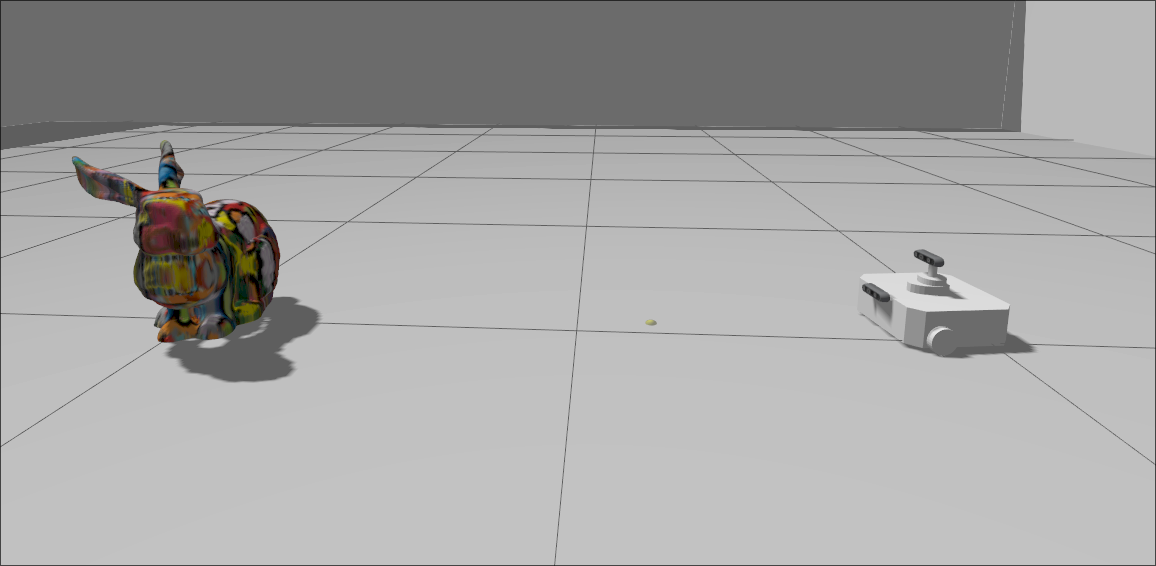
\includegraphics[width=0.5\textwidth]{Graphics/tbandbunny.png}

	\today
\end{frame}

\section{Allgemeines}
\begin{frame}{Motivation}
	\begin{minipage}{0.55 \textwidth}
		\begin{block}{Ziel}
			\begin{itemize}
				\item autonom Bilder von Objekt aufnehmen
				\item Bilder aus verschiedenen Perspektiven
				\item Bilder als Training für Perzeptionsmodellen
				\item Soll auf verschiedenen Robotern laufen (Spot, Turtlebot, etc.)
			\end{itemize}
		\end{block}
	\end{minipage}
	\hfill
	\begin{minipage}{0.4 \textwidth}
		\centering
		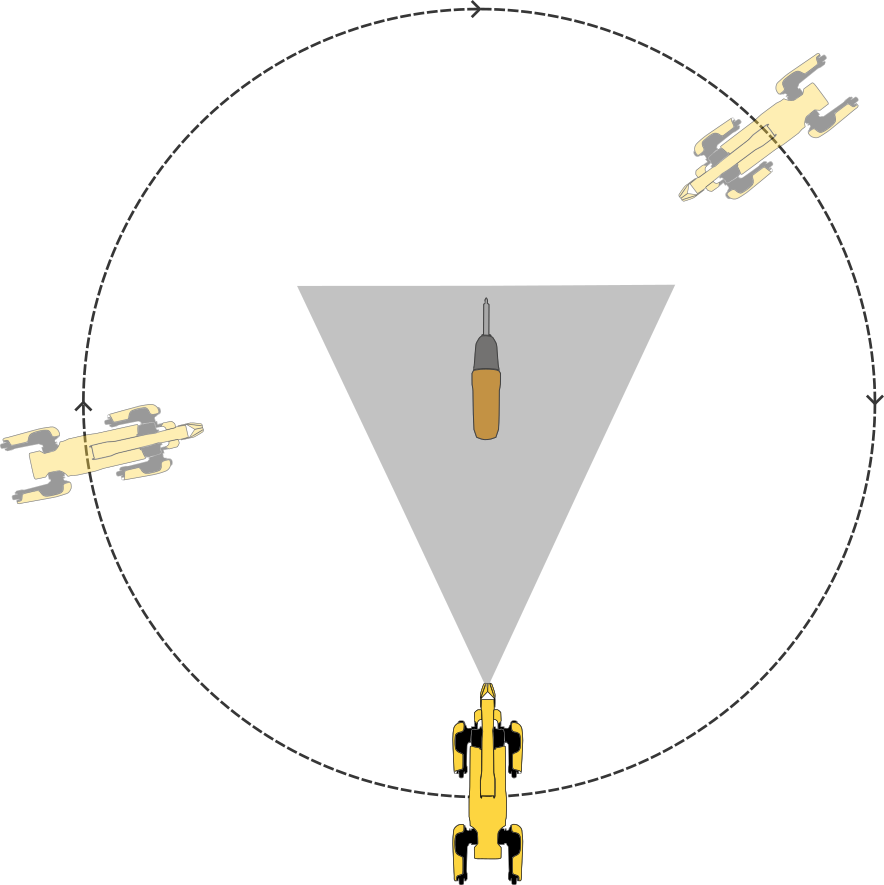
\includegraphics[width=1\textwidth]{Graphics/graphic_top_down.png}
	\end{minipage}
\end{frame}

\begin{frame}{State of the Art}
	\begin{center}
		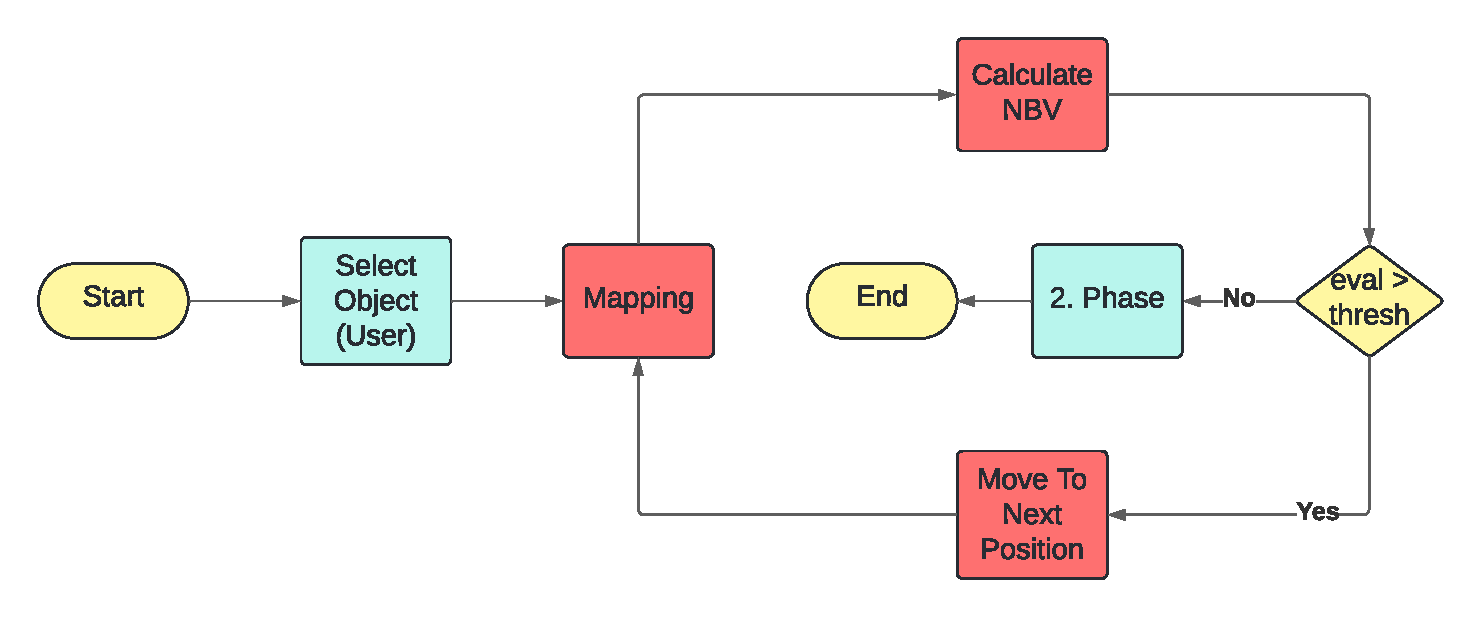
\includegraphics[width=0.65\textwidth]{Graphics/flow_chart.pdf}
	\end{center}

	\begin{block}{}
		\begin{itemize}
			\item Mögliche Positionen evaluieren
			\item Abschätzen wie viel Informationen in möglicher Position gesehen wird (Next-Best-View)
			\item Andere Faktoren für Positionen evaluieren (Distanz, Überlappung, Sichtbarkeit des Bekannten etc.)
			\item Zur besten Position gehen
		\end{itemize}
	\end{block}
\end{frame}

\section{State of the Art}
\begin{frame}{State of the Art: NBV}
	\vspace{-1cm}
	\hfill
	\begin{minipage}{0.2\textwidth}
		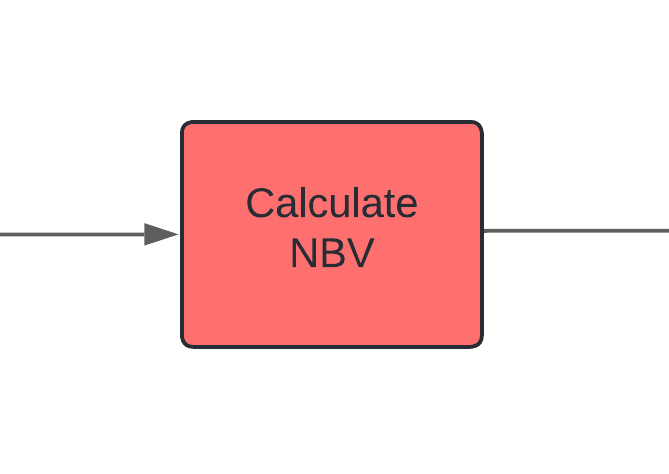
\includegraphics[width=\textwidth]{Graphics/nbv_flow.png}
	\end{minipage}
	\vspace{-0.5cm}
	\begin{block}{Klassische Ansätze}
		\begin{itemize}
			\item \textbf{Annahme:} Tiefensensor, Größe des Objekts bekannt (Bounding Box)
			\item Generierung von Kandidaten Sensorpose, meist auf Kugel um Objektzentrum
			\item Testen der Kandidaten auf \textbf{utility function}
			\item Zur besten Kandidaten Sensorpose bewegen
			\item \textbf{Repräsentation der Umgebung:} OctoMap, ähnliche Voxelkarten
		\end{itemize}
		\cite{zeng_view_2020}
	\end{block}
	\begin{textblock*}{0.2\textwidth}(10cm, 6.5cm)
		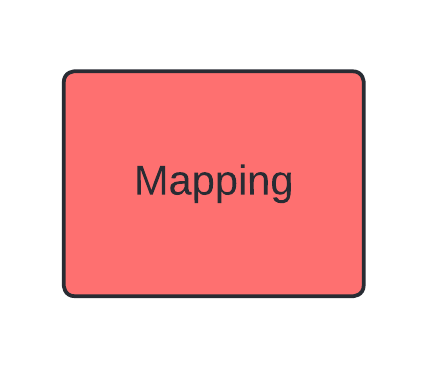
\includegraphics[width=\textwidth]{Graphics/mapping_flow.png}
	\end{textblock*}
\end{frame}

\begin{frame}{State of the Art: NBV}
	\vspace{-1cm}
	\hfill
	\begin{minipage}{0.2\textwidth}
		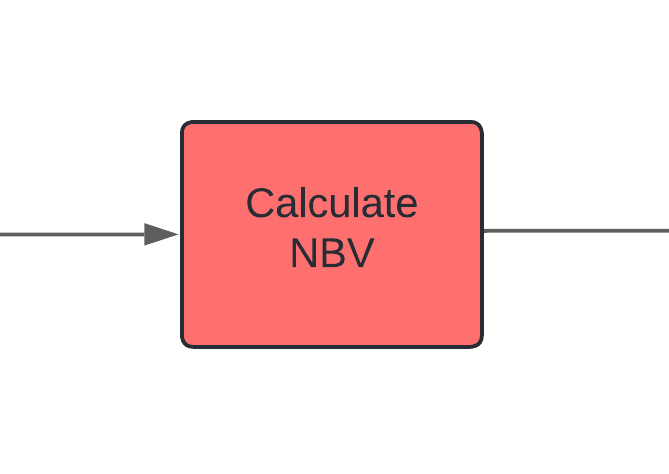
\includegraphics[width=\textwidth]{Graphics/nbv_flow.png}
	\end{minipage}
	\vspace{-0.5cm}
	\begin{block}{Machine-Learning Ansätze}
		\begin{itemize}
			\item \textbf{Annahme:} Trainingsdaten auf Basis von Punktwolke oder Voxelkarte
			\item Trainingsdaten enthalten nächst-beste Sensorpose für aktuelle Sensorpose
			\item Nächste Sensorpose vorhersagen
			\item PC-NBV \cite{zeng_pc-nbv_2020}, NBV-Net \cite{mendoza_supervised_2020}

		\end{itemize}
	\end{block}
\end{frame}

\begin{frame}{State of the Art: Definitionen}
	\begin{exampleblock}{Visible unknown voxel (VUV)}
		\begin{itemize}
			\item unbekannte Voxel, die von einem anderen Punkt als erste gesehen werden
			\item unbekannte Voxel benachbart zu einem freien Voxel
		\end{itemize}
		\cite{vasquez-gomez_vpl_2020}
	\end{exampleblock}
	\begin{exampleblock}{Frontier voxel}
		\begin{itemize}
			\item visible unknown Voxel, die benachbart zu besetzen Voxel sind
			\item benachbarte Frontier Voxel bilden eine Frontier

		\end{itemize}
		\cite{vasquez-gomez_vpl_2020}
	\end{exampleblock}
\end{frame}

\begin{frame}{State of the Art}
	\begin{figure}
		\hspace{2.2cm}
		\begin{tikzpicture}
			% Centered image
			\node (main-image) at (current page.center) {
				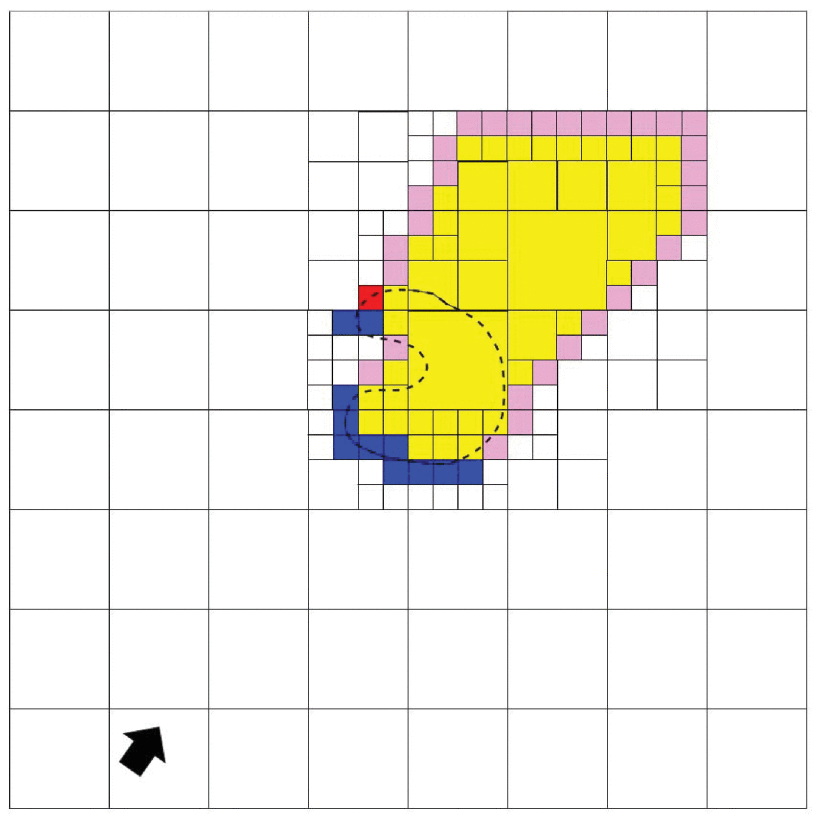
\includegraphics[width=6cm]{Graphics/vasquez.png} % Adjust width
			};
			% Secondary image at the top right of the centered image
			\node[xshift=1.5cm, yshift=-0.9cm]
			(secondary-image) at (main-image.north east){
				
\includegraphics[width=3cm]{Graphics/legend.png} % Smaller image
			};
		\end{tikzpicture}
		\caption{ Abbildung von Vasquez-Gomez et al. \cite{vasquez-gomez_vpl_2020}}
	\end{figure}
\end{frame}


\begin{frame}{Ansatz}
	\begin{block}{Besonderheiten}
		\begin{itemize}
			\item keine Information über Größe des Objekts
			\item VDB-Mapping statt OctoMap
		\end{itemize}
	\end{block}
	\begin{exampleblock}{}
		Solange bis der Informationsgewinn vernachlässigbar ist
		\begin{enumerate}
			\item Oberflächen-Voxel und Frontier Voxel finden
			\item Frontiers gruppieren
			\item Kandidaten generieren
			\item Kandidaten evaluieren und besten Kandidaten finden
		\end{enumerate}
	\end{exampleblock}


	\begin{textblock*}{0.2\textwidth}(10cm, 3.6cm)
		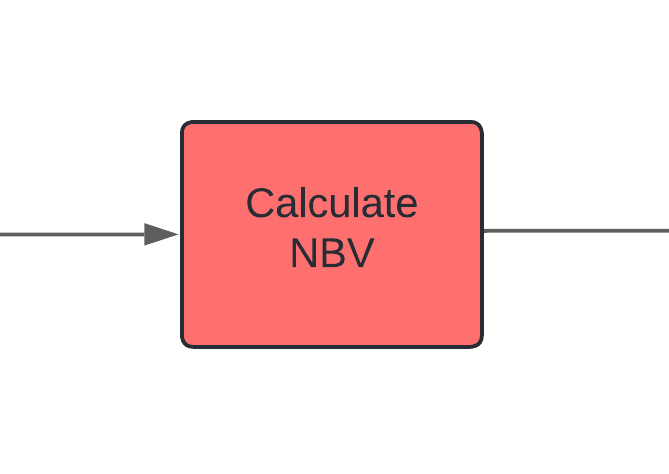
\includegraphics[width=\textwidth]{Graphics/nbv_flow.png}
	\end{textblock*}

\end{frame}

\begin{frame}{Ansatz}
	\begin{minipage}{0.59\textwidth}
		\begin{block}{Zweite Phase}
			\begin{itemize}
				\item Tiefeninformation $\neq$ Bilder
				\item Algorithmus hört häufig auf bevor Objekt von allen Seiten gesehen wurde
				\item Zweite Phase, die Lücken füllt
				\item \textbf{Annahme:} Durch erste Phase sind grobe Dimensionen bekannt
			\end{itemize}
		\end{block}
	\end{minipage}
	\begin{minipage}{0.4\textwidth}
		\centering
		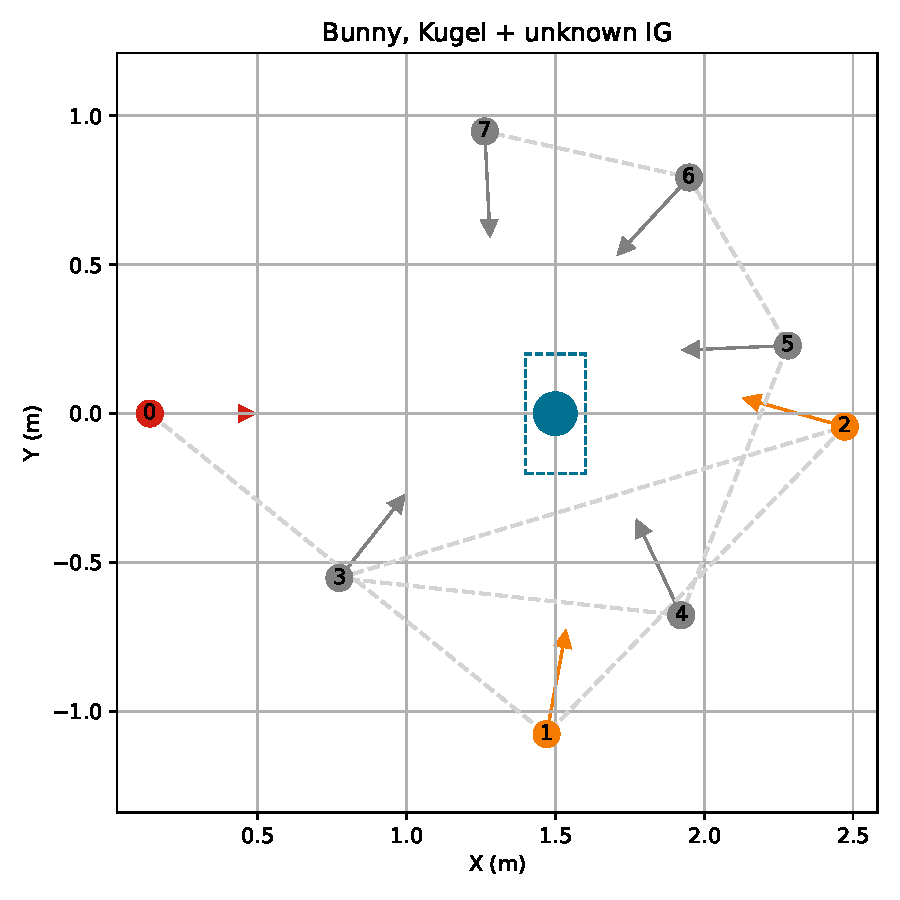
\includegraphics[width=1\textwidth]{Graphics/bunny_sphere_unknown_views.pdf}
	\end{minipage}
\end{frame}


\begin{frame}{Erste Phase: Schritt 1 \& 2}

	\begin{block}{1. Breitensuche: Frontier-Voxel und Oberflächen-Voxel}
		\begin{itemize}
			\item Finde alle besetzen Voxel, die über besetze Voxel mit Ursprung verbunden sind
			\item Findet die bisher bekannte Oberfläche
			\item Filtert den Boden heraus
			\item Markiert alle gefundenen unbekannte Voxel die freien Nachbarn haben
		\end{itemize}
	\end{block}
	\begin{exampleblock}{2. Breitensuche: Frontier Voxel gruppieren}
		\begin{itemize}
			\item 2 verschachtelte Breitensuchen
			\item gruppiert alle benachbarten Frontier Voxel zu einer Frontier
			\item Berechnet Zentrum der Frontier
		\end{itemize}
	\end{exampleblock}
\end{frame}

\begin{frame}{Schritt 1 \& 2}
	\vspace{-0.4cm}
	\begin{figure}
		\centering
		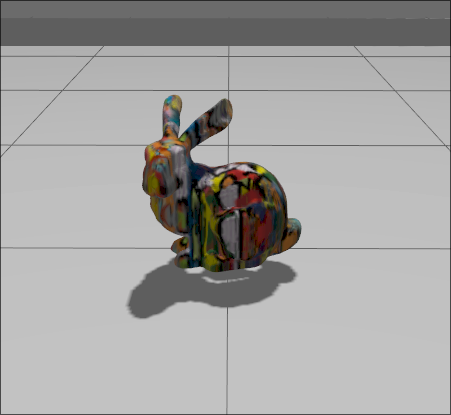
\includegraphics[width=0.35\textwidth]{Graphics/bunny.png}
		\caption{Bunny collada Datei von \cite{delmerico_comparison_2018}}
	\end{figure}
	\vspace{-0.2cm}
	\centering
	\begin{minipage}{0.4\textwidth}
		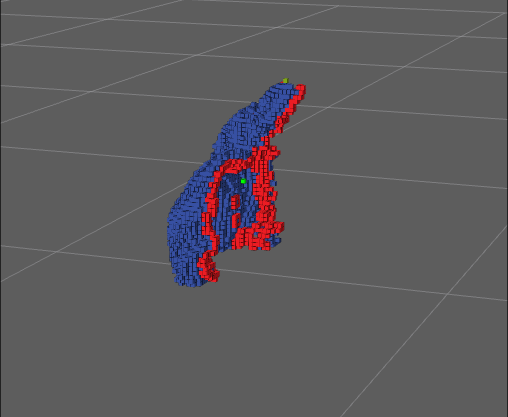
\includegraphics[width=\textwidth]{Graphics/frontiers_side.png}
	\end{minipage}
	%\end{center}
	%\hfill
	\begin{minipage}{0.4\textwidth}
		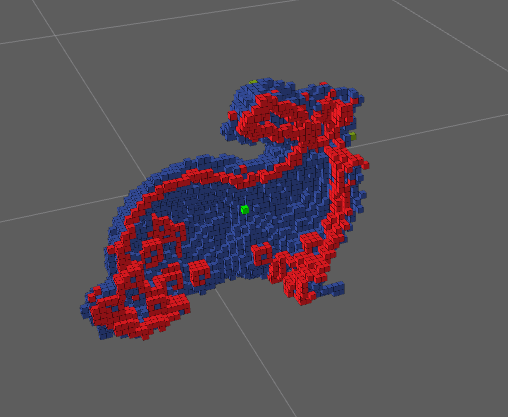
\includegraphics[width=\textwidth]{Graphics/frontiers_behind.png}
	\end{minipage}

\end{frame}
\begin{frame}{Schritt 3: Kandidaten Positionen generieren}
	\begin{block}{}

		\begin{center}
			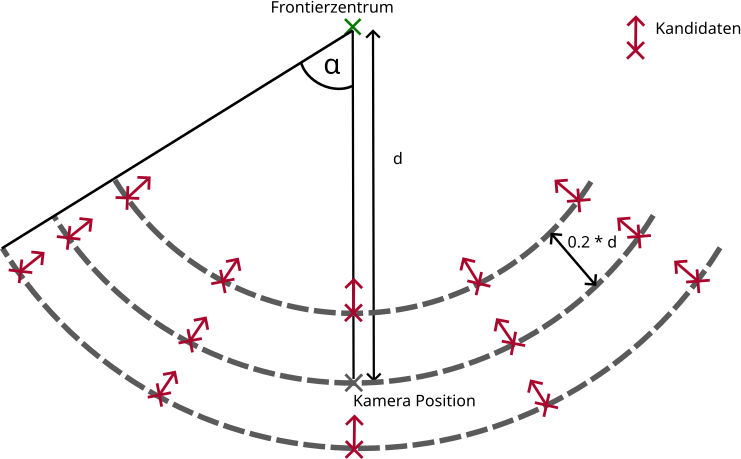
\includegraphics[width=0.7\textwidth]{Graphics/view_point_gen_v2.png}
		\end{center}
		\begin{itemize}
			\item Sampling zwischen fixen Distanzen, abhängig von aktueller Distanz $d$
			\item Sampling zwischen maximalem Ausschlagswinkel $\alpha$
			\item Alle Kandidaten werden evaluiert
		\end{itemize}
	\end{block}

\end{frame}

\begin{frame}{Schritt 4: Informationsgewinn}
	\begin{block}{Informationsgewinn abschätzen}
		Informationsgewinn abschätzen:
		\begin{itemize}
			\item Ray tracing durch die VDB map von der Kandidatenpose
			\item Strahlen gehen durch alle Pixel der Ausgabe (640x480)
			\item Strahlen verfolgen bis besetzter Voxel getroffen wird
			\item Zwei Möglichkeiten für unbekannte Voxel: \begin{itemize}
				      \item Strahlenverfolgung stoppen wenn unbekannter Voxel getroffen wird (VUV IG)
				      \item Strahlen weiter verfolgen und alle unbekannten Voxel zählen (Unknown IG)
			      \end{itemize}
		\end{itemize}

	\end{block}

\end{frame}

\begin{frame}{Informationsgewinn: Unknown Barrier}
	\begin{block}{}
		\begin{center}
			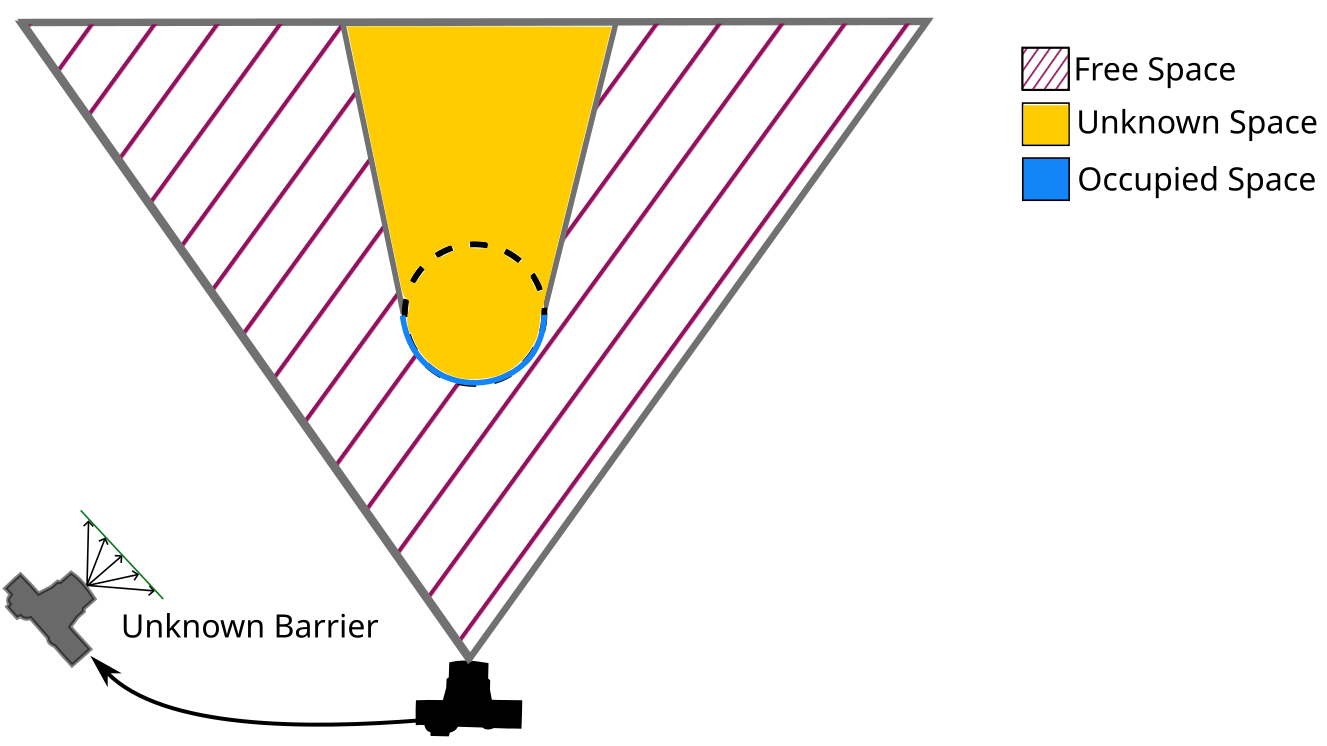
\includegraphics[width=0.7\textwidth]{Graphics/unknown_barrier_vscott_1.png}
		\end{center}
		\begin{itemize}
			\item Alle Strahlen von neuer Kamera Position treffen auf unbekannte Voxel
			\item Interessanter Bereich hinter Object minimieren
		\end{itemize}
	\end{block}
\end{frame}

\begin{frame}{Informationsgewinn: Unknown Barrier}
	\begin{block}{}
		\begin{center}
			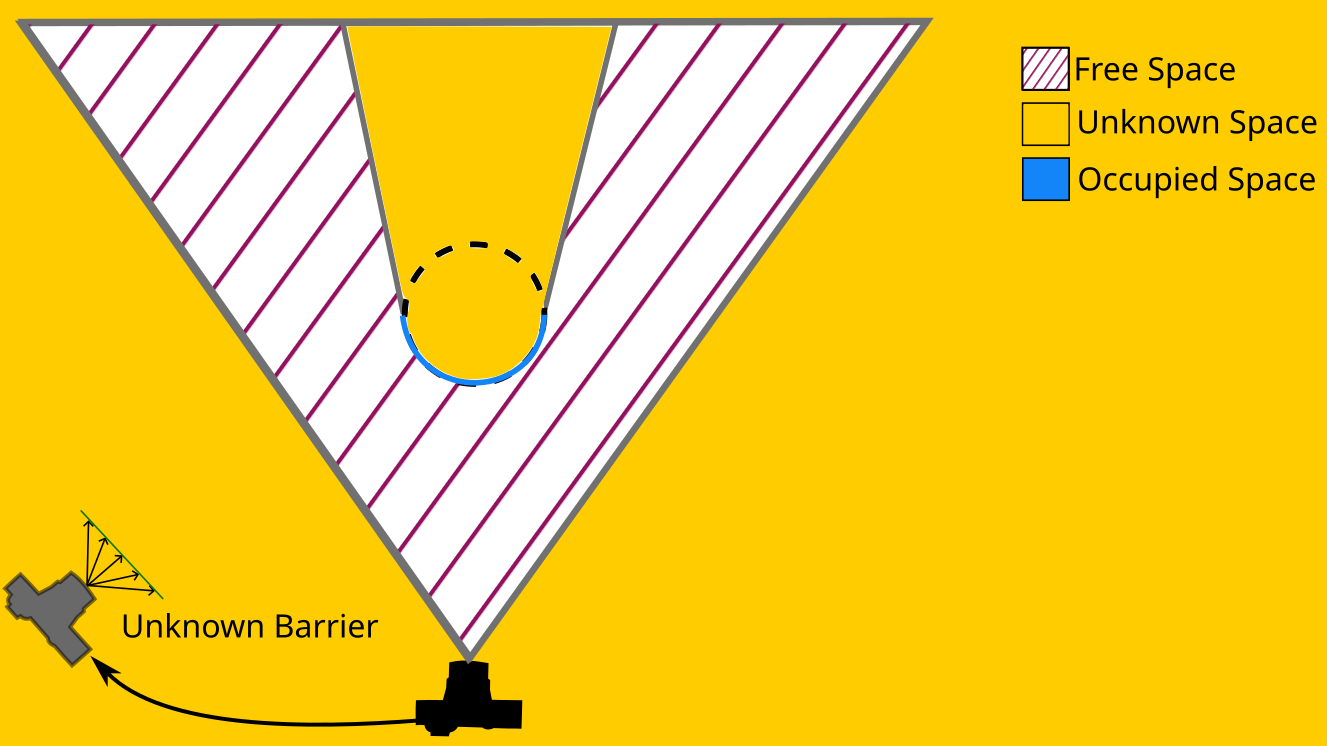
\includegraphics[width=0.7\textwidth]{Graphics/unknown_barrier_vscott_2.png}
		\end{center}
		\begin{itemize}
			\item Alle Strahlen von neuer Kamera Position treffen auf unbekannte Voxel
			\item Interessanter Bereich hinter Object minimieren
		\end{itemize}
	\end{block}
\end{frame}

\begin{frame}{Informationsgewinn: Heuristiken}
	\begin{block}{\textbf{1. Lösung:} Kugel}
		\begin{center}
			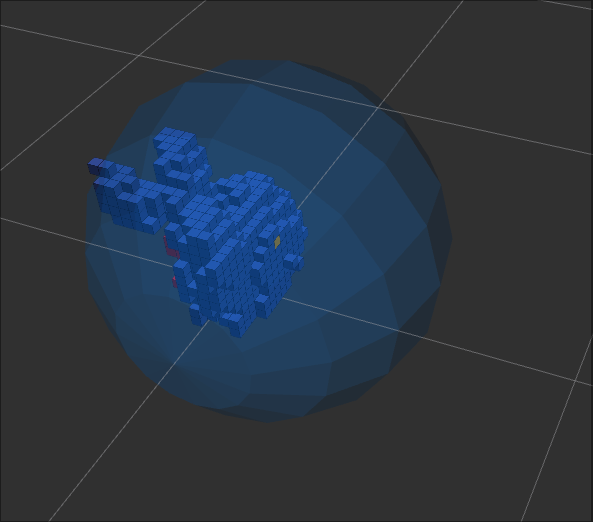
\includegraphics[width=0.4\textwidth]{Graphics/sphere.png}
		\end{center}
		\begin{itemize}
			\item  Kugel um Ursprung mit Radius maximal Abstand zu einem Oberflächenvoxel
			\item \textbf{Vorteil:} Einfaches ray tracing, einfach zu berechnende Heuristik
		\end{itemize}
	\end{block}
\end{frame}

\begin{frame}{Informationsgewinn: Heuristiken}
	\begin{block}{\textbf{1. Lösung:} Kugel}
		\begin{center}
			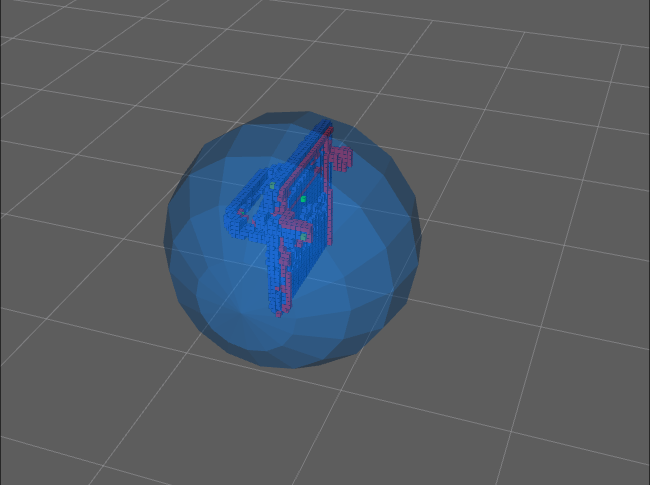
\includegraphics[width=0.4\textwidth]{Graphics/sphere_ok.png}
			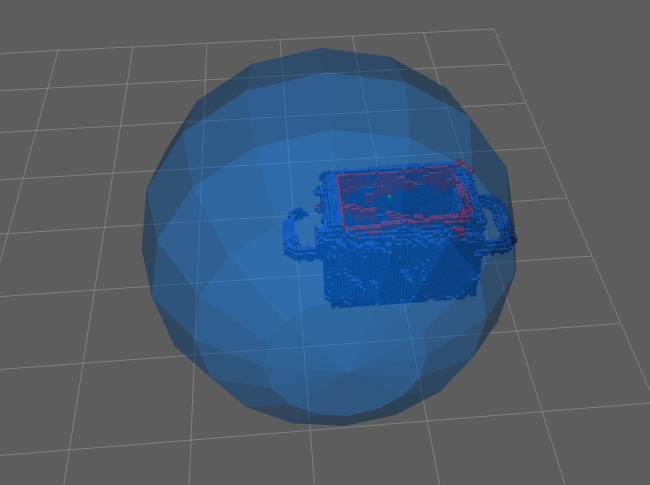
\includegraphics[width=0.4\textwidth]{Graphics/sphere_too_big.png}
		\end{center}
		\begin{itemize}
			\item Kugel um Ursprung mit Radius maximal Abstand zu einem Oberflächenvoxel
			\item \textbf{Vorteil:} Einfaches ray tracing, einfach zu berechnende Heuristik
			\item \textbf{Nachteil: Ungeeignet vor allem für unsymmetrische Objekte}
		\end{itemize}
	\end{block}
\end{frame}

\begin{frame}{Informationsgewinn: Heuristiken}
	\begin{block}{\textbf{2. Lösung:} Frustum}
		\begin{center}
			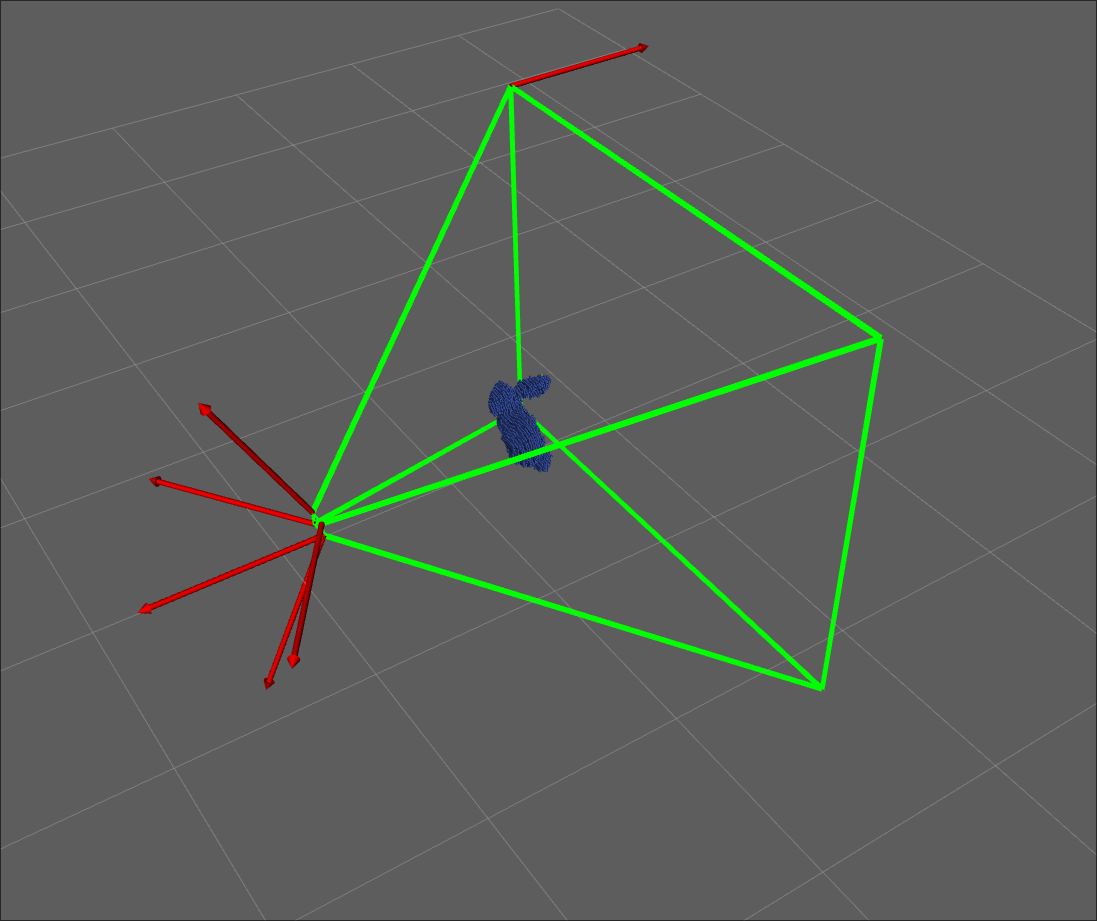
\includegraphics[width=0.5\textwidth]{Graphics/frustum_2.png}
		\end{center}
		\begin{itemize}
			\item Aktueller Sichtkörper der Kamera (View Frustum)
		\end{itemize}
	\end{block}
\end{frame}

\begin{frame}{Informationsgewinn: Heuristiken}

	\begin{exampleblock}{\textbf{2. Lösung:} Frustum: Vor- und Nachteile}
		\begin{itemize}
			\item \textbf{Vorteil:} Im allgemeinen weniger falsch-ausgeschlossene Voxel
			\item \textbf{Nachteile:} \begin{itemize}
				      \item Sehr großer Bereich zur Suche $\rightarrow$ höhere Laufzeit
				      \item Voxel hinter initialer Kameraposition sind unbekannt \\ $\rightarrow$ zweites lokales Maximum von unbekannten Voxeln
			      \end{itemize}
		\end{itemize}
	\end{exampleblock}
\end{frame}

\begin{frame}{Informationsgewinn: Heuristiken}
	\begin{block}{\textbf{3. Lösung:} Reduced Frustum}
		\begin{center}
			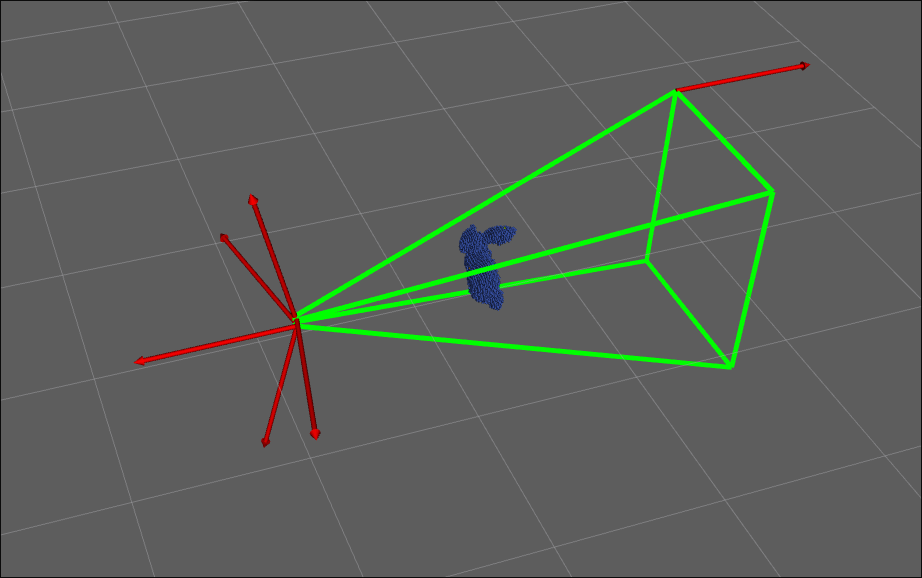
\includegraphics[width=0.4\textwidth]{Graphics/reduced_frustum.png}
		\end{center}
		\begin{itemize}
			\item Aktueller Sichtkörper der Kamera reduziert auf das Objekt (Reduced Frustum)
			\item \textbf{Vorteil:} Im allgemeinen weiniger falsch-ausgeschlossene Voxel \& kleiner als Sichtkörper
			\item \textbf{Nachteil:} Voxel hinter initialer Kameraposition sind unbekannt
		\end{itemize}
	\end{block}
\end{frame}

\begin{frame}{Sichtkörper: Zweites Maximum}
	\center
	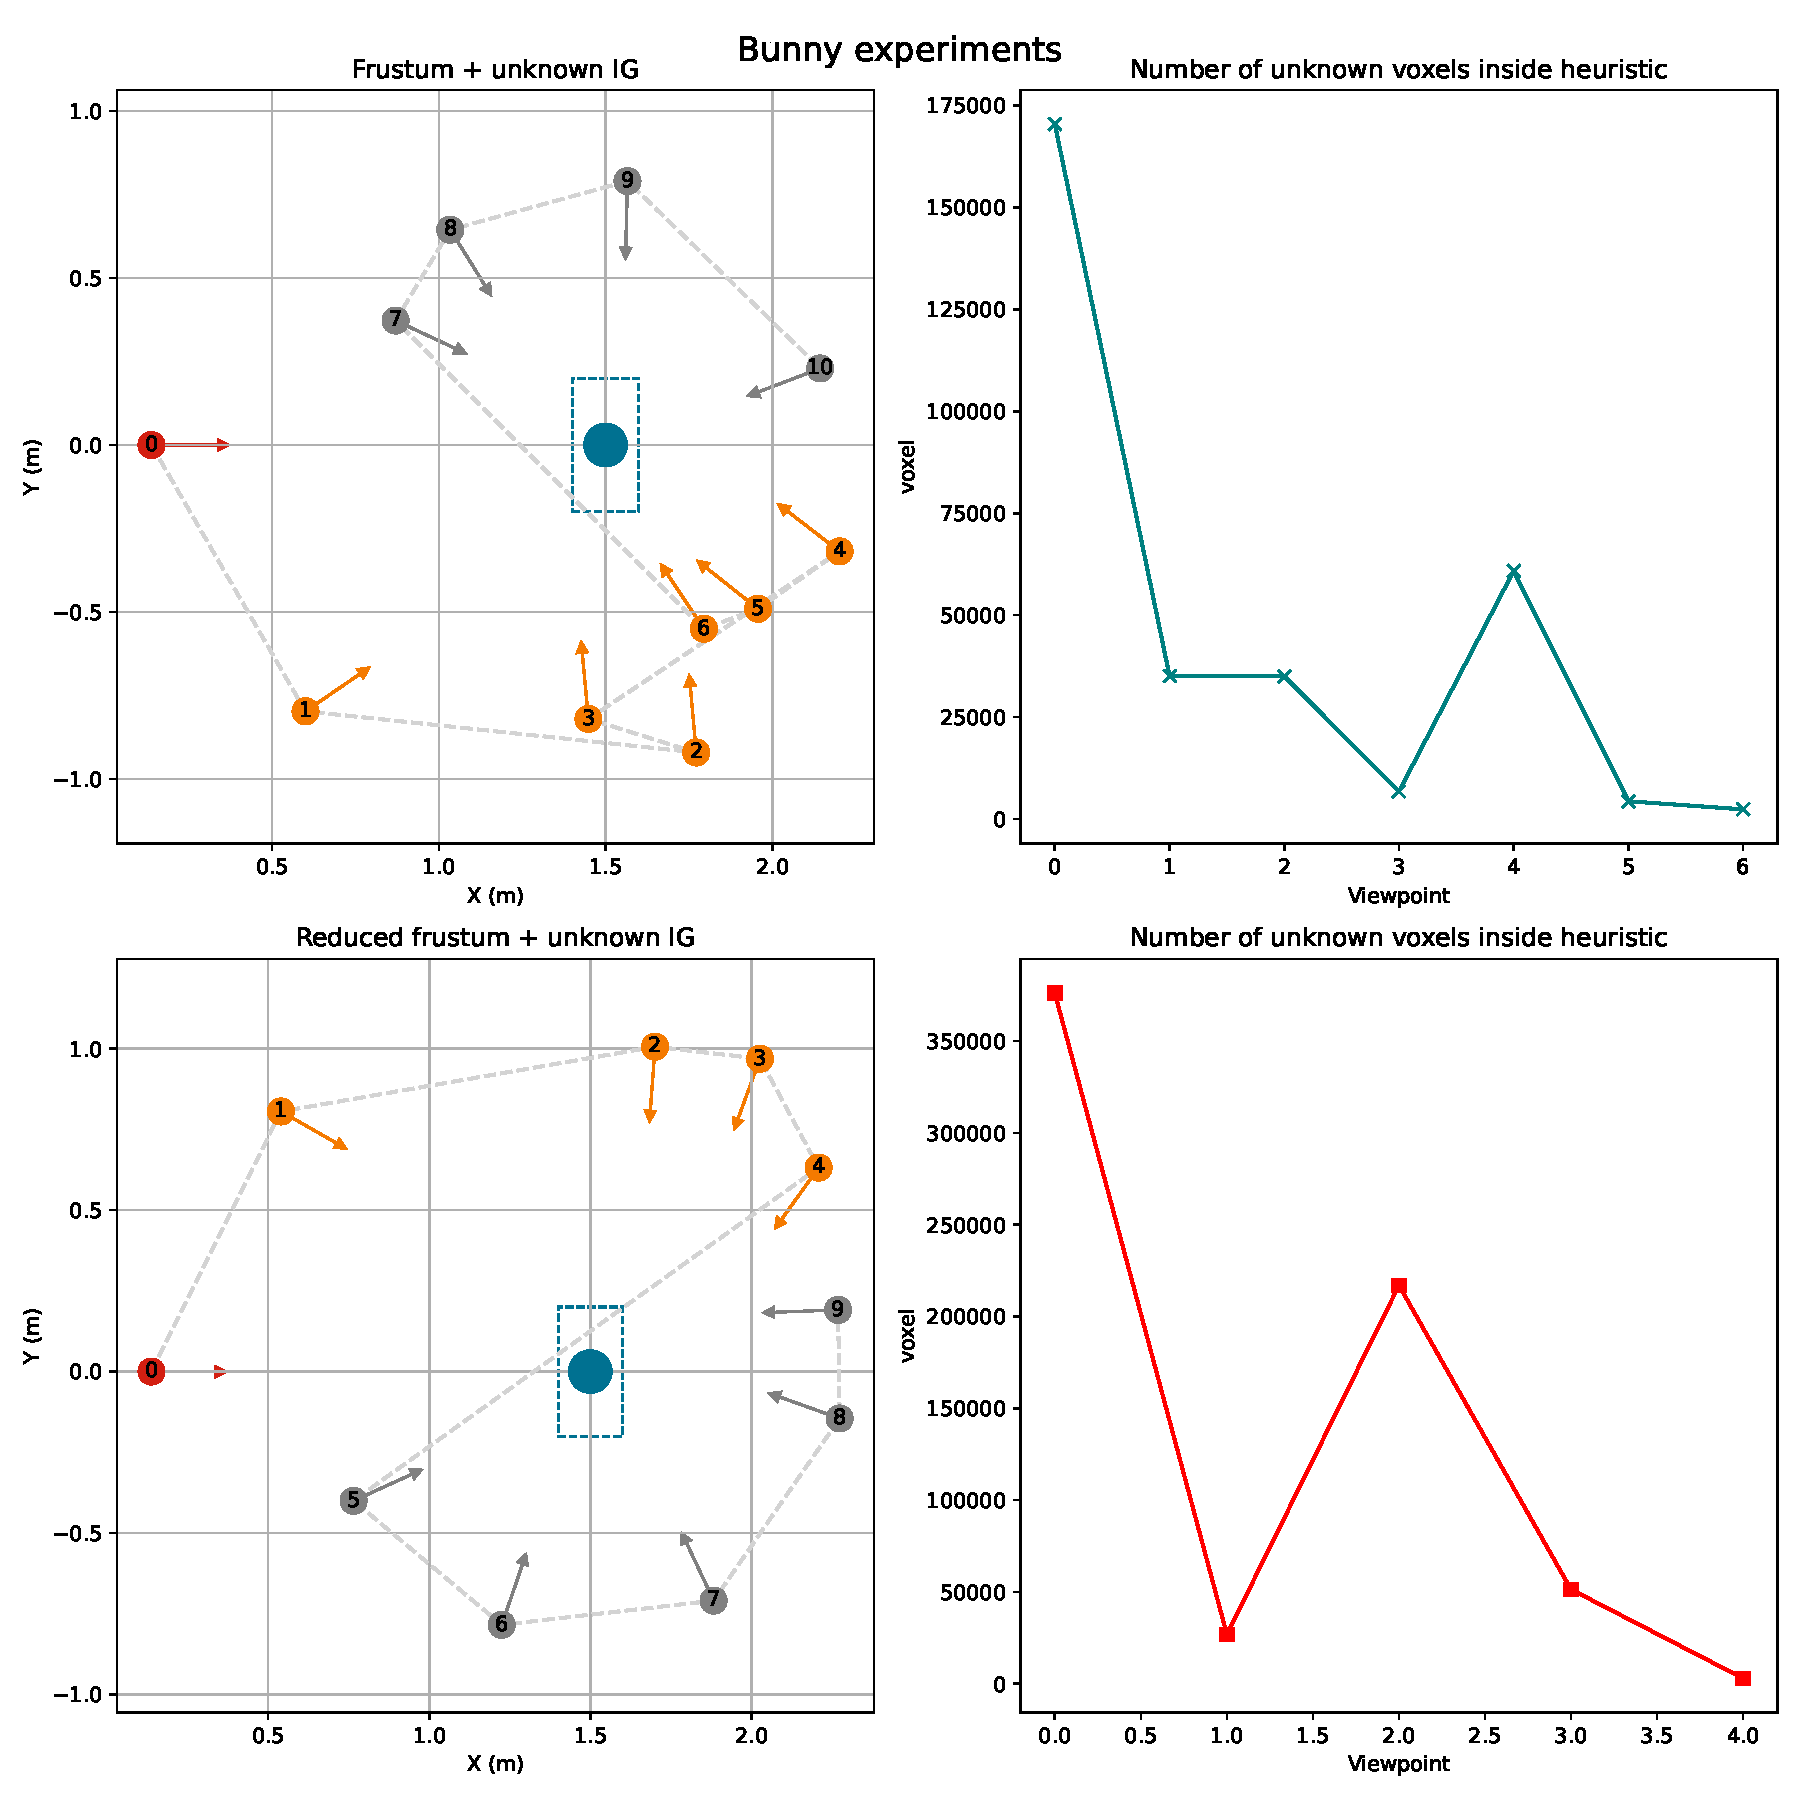
\includegraphics[width=0.65\textwidth]{Graphics/bunny_views_unknown_voxels.pdf}
\end{frame}

\begin{frame}{Schritt 4: Utility Function}

	\begin{exampleblock}{Informationsgewinn}
		Kombination aus Heuristiken und Informationsgewinn Strategien ergibt 6 Metriken:
		\\ \{Kugel, Sichtkörper, Reduzierter Sichtkörper\} $\times$ \{VUV, Unknown\}
	\end{exampleblock}
	\begin{block}{Utility Function}
		Folgende Faktoren werden für die Utility Function gewertet:
		\begin{itemize}
			\item $I(v)$ Informationsgewinn, durch ray tracing bestimmt (Metriken siehe oben)
			\item $c(v)$ Cut-off Faktor, um abgeschnittene Bilder zu verhindern
			\item $d(v)$ Distanz zur Kandidatenpose
			\item $p(v) \in \{0,1\}$ Erreichbarkeit der Kandidatenpose
			\item $F(v)$ Frontier Faktor
		\end{itemize}
	\end{block}
\end{frame}

\section{Experimente}
\begin{frame}{Utility Function: Initialer Blickwinkel von der Kiste}
	\centering
	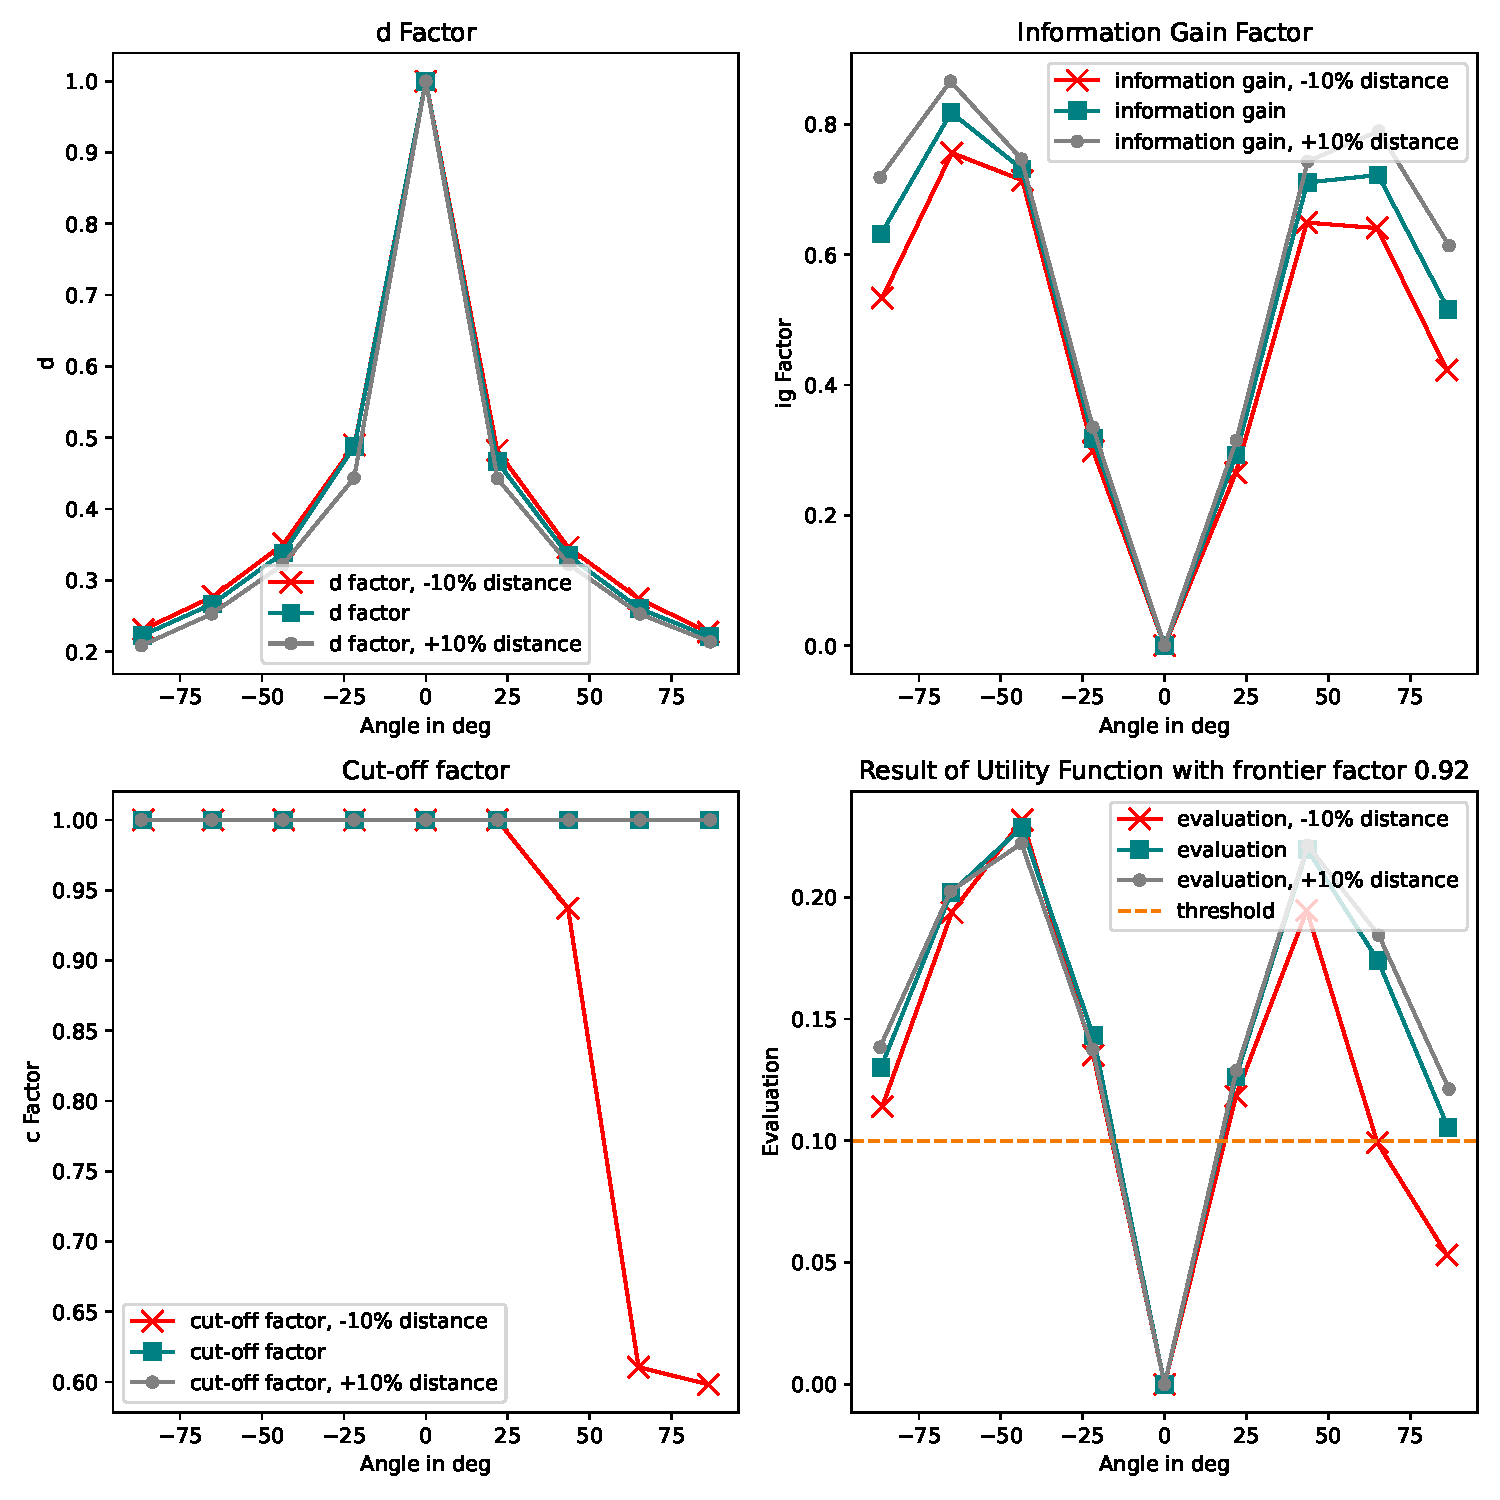
\includegraphics[width=0.65\textwidth]{Graphics/crate_allinone_first.pdf}
\end{frame}

%\begin{frame}{Utility Function: Letzter Blickwinkel von der Kiste}
%	\centering
%	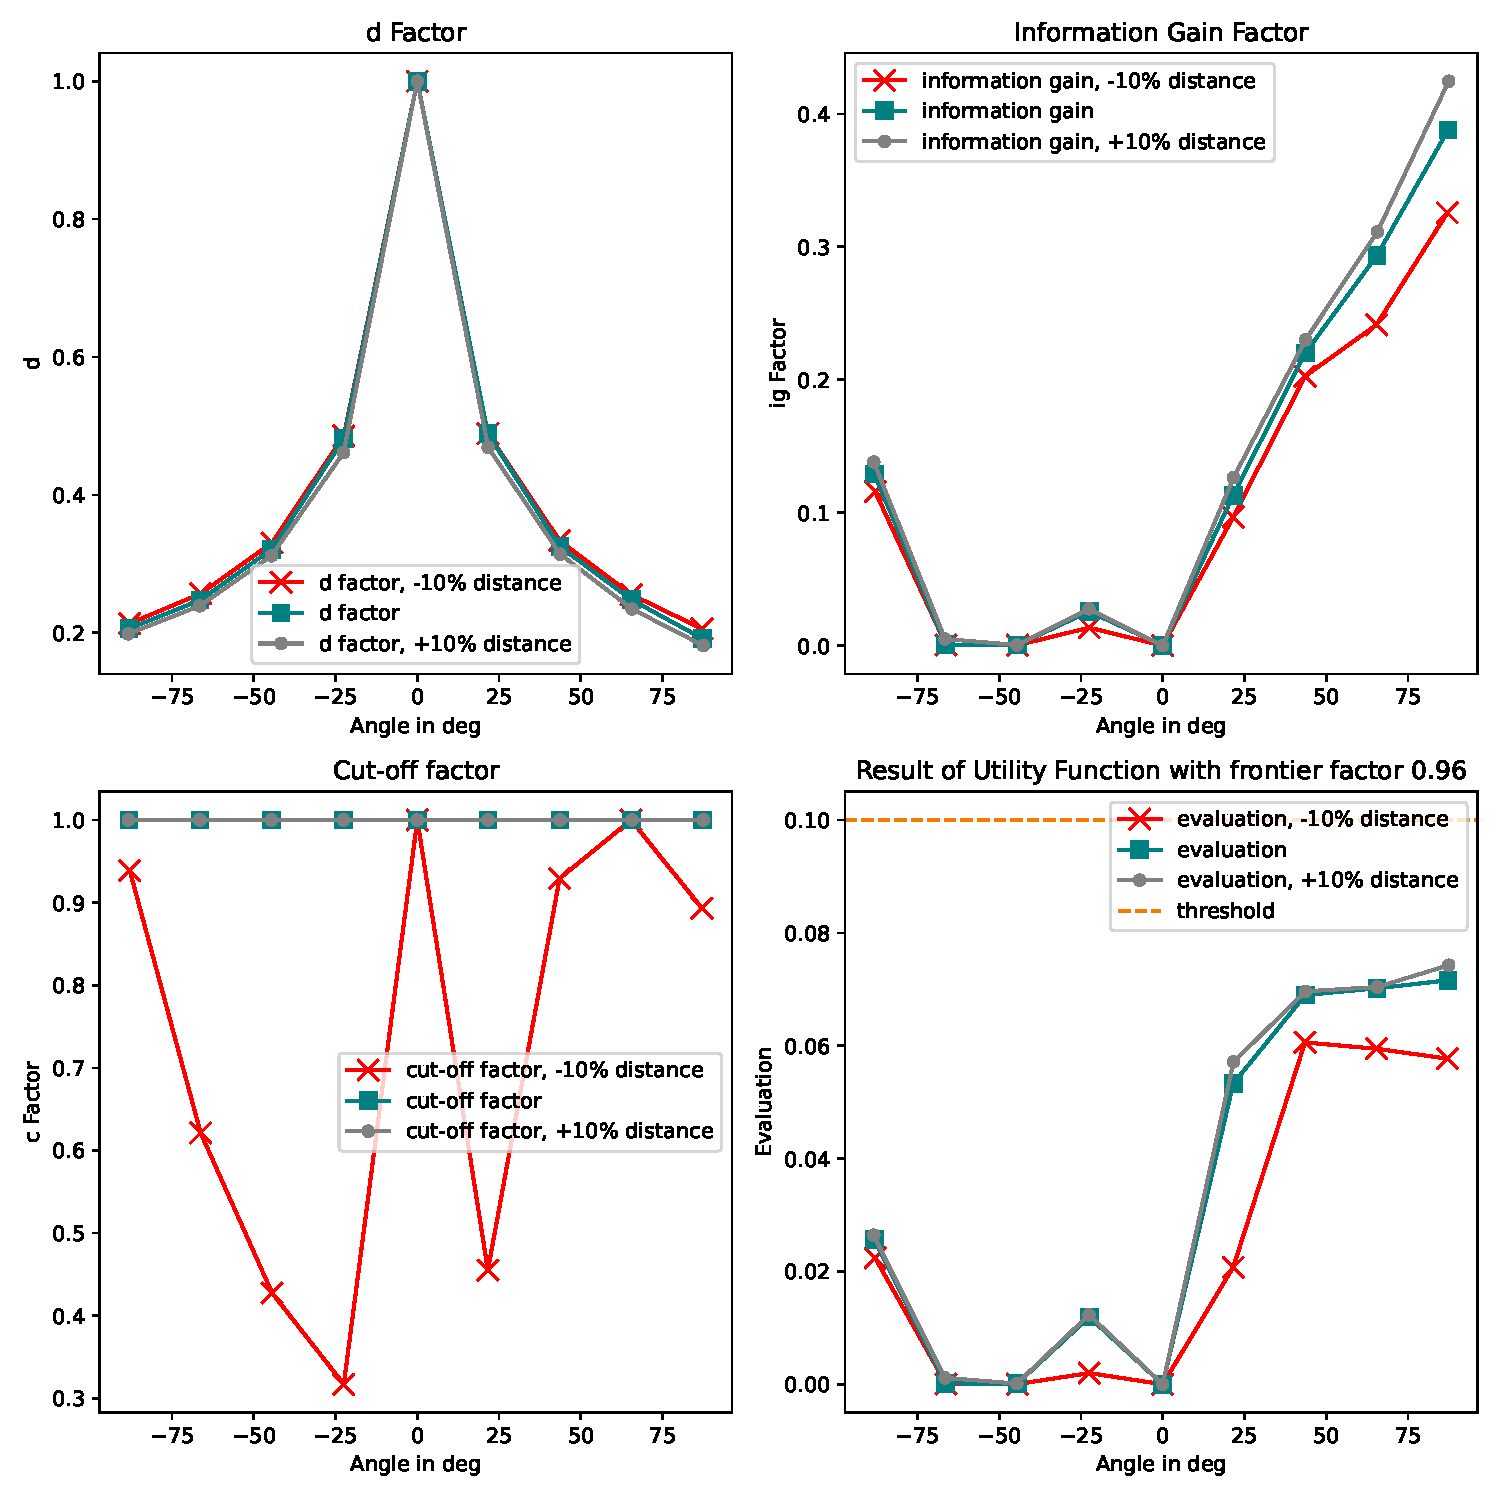
\includegraphics[width=0.65\textwidth]{Graphics/crate_allinone_last.pdf}
%\end{frame}

\begin{frame}{Experimente: Objekte}

	\begin{figure}[h]
		\centering
		\begin{subfigure}{0.45\textwidth}
			\centering
			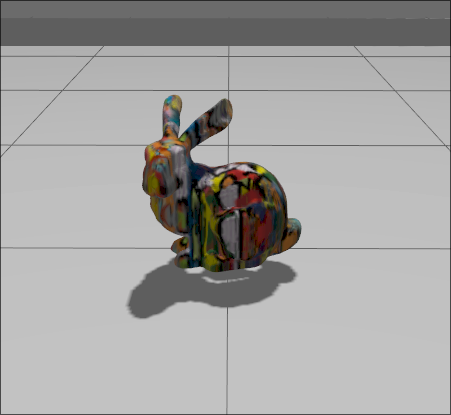
\includegraphics[width=0.8\textwidth]{Graphics/bunny.png}
			\caption{Bunny von \cite{noauthor_stanford_nodate}, Model von \cite{delmerico_comparison_2018}}
		\end{subfigure}
		\begin{subfigure}{0.45\textwidth}
			\centering
			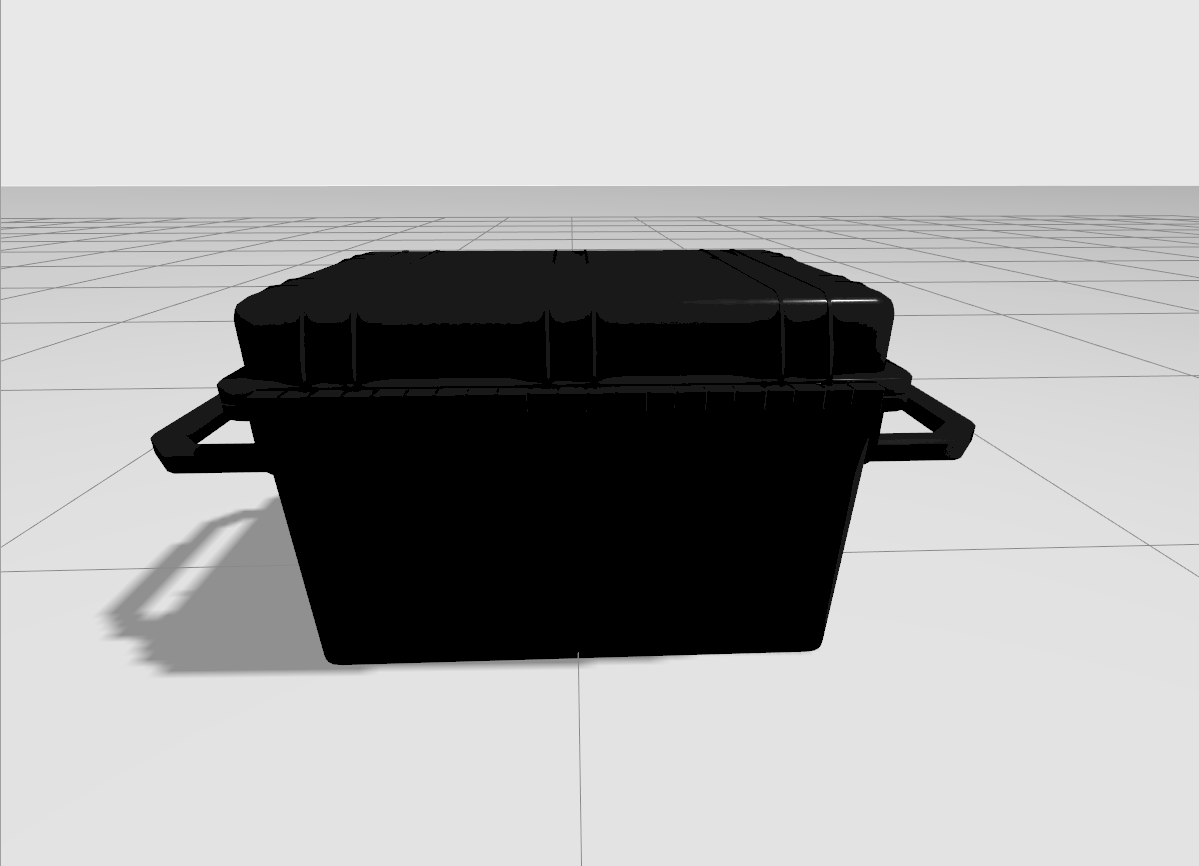
\includegraphics[width=0.8\textwidth]{Graphics/crate}
			\caption{Schwarze Kiste von \cite{GazeboFuel-OpenRobotics-Large-Crate}}
		\end{subfigure}
		\vspace{0.5cm}
		\begin{subfigure}{0.45\textwidth}
			\centering
			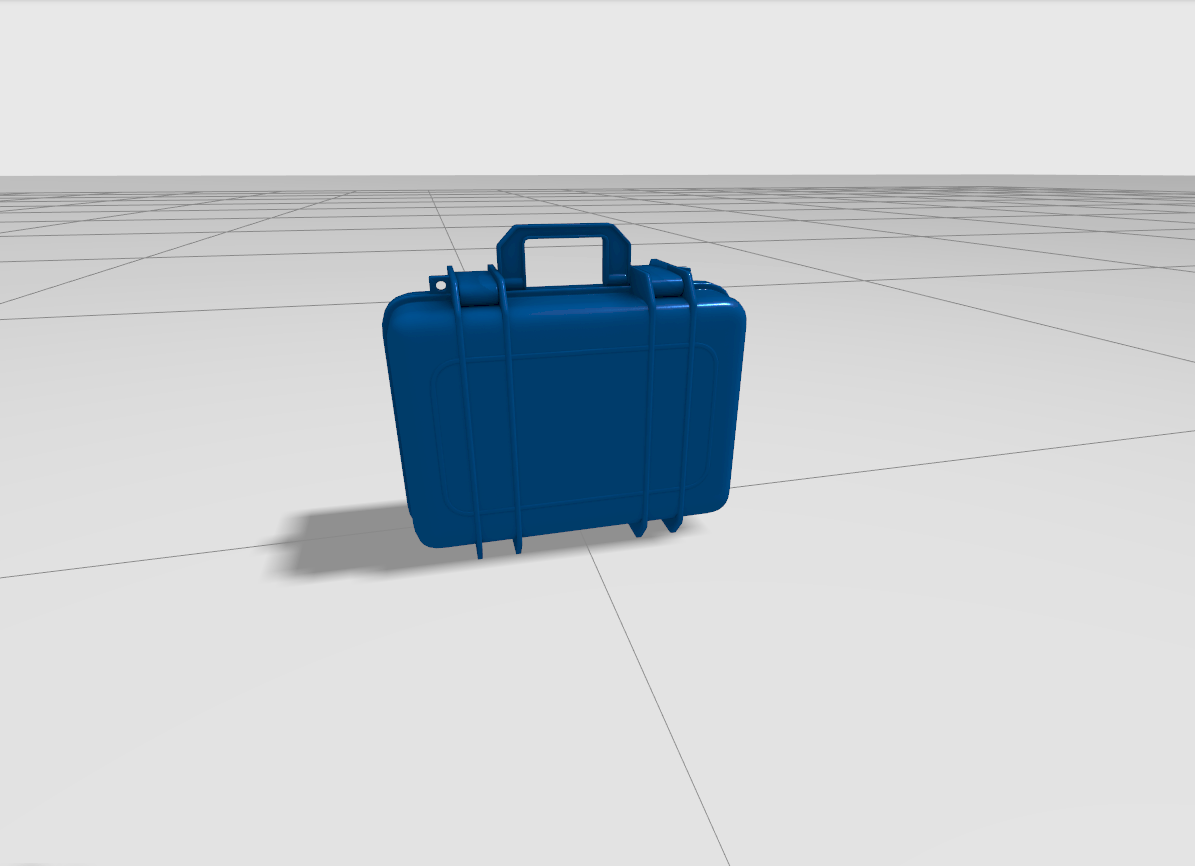
\includegraphics[width=0.8\textwidth]{Graphics/box}
			\caption{Kleine blaue Box von \cite{GazeboFuel-OpenRobotics-Small-Blue-Box}}
		\end{subfigure}
		\begin{subfigure}{0.45\textwidth}
			\centering
			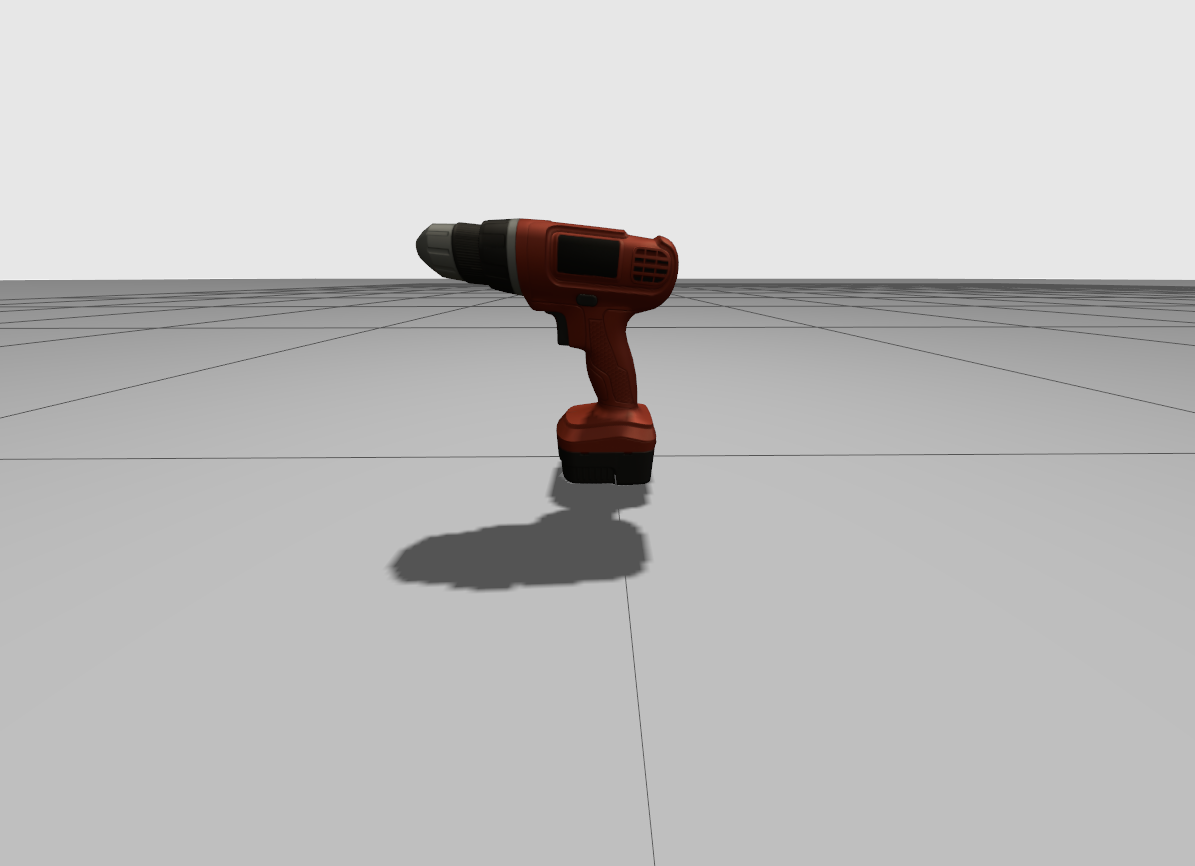
\includegraphics[width=0.8\textwidth]{Graphics/drill}
			\caption{Bohrmaschine von \cite{GazeboFuel-OpenRobotics-Black-and-Decker-Cordless-Drill}}
		\end{subfigure}
	\end{figure}

\end{frame}

\begin{frame}{Experimente: Ergebnisse}
	\centering
	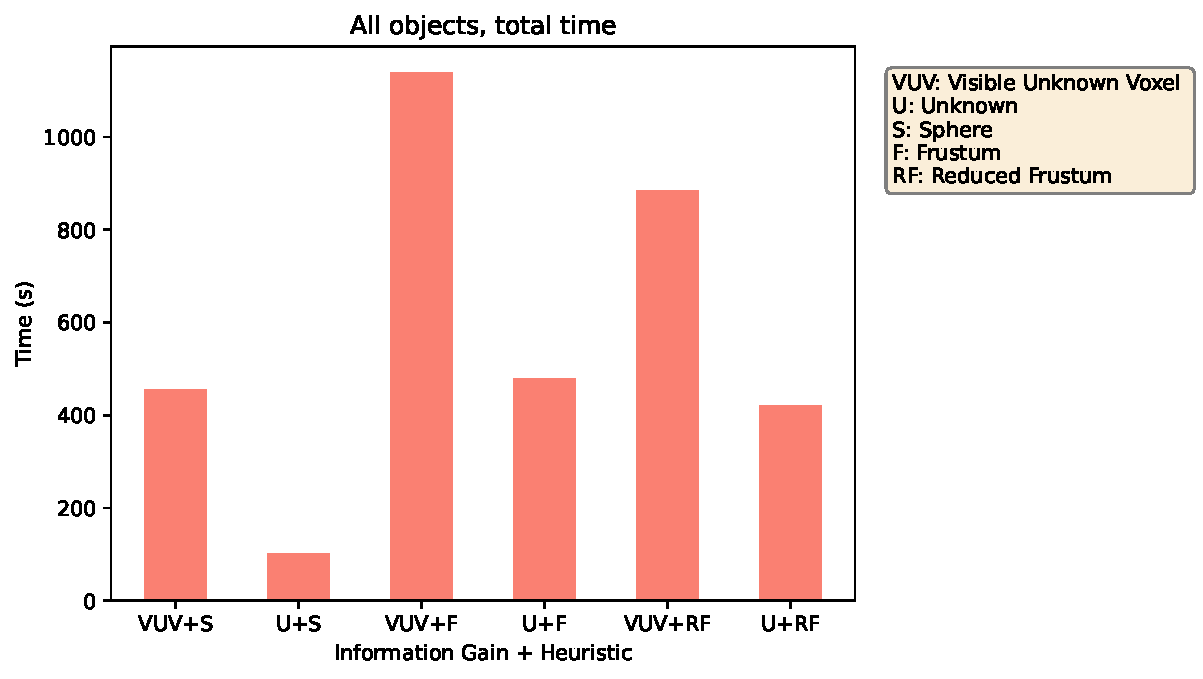
\includegraphics[width=0.6\textwidth]{Graphics/all_total_times.pdf}
	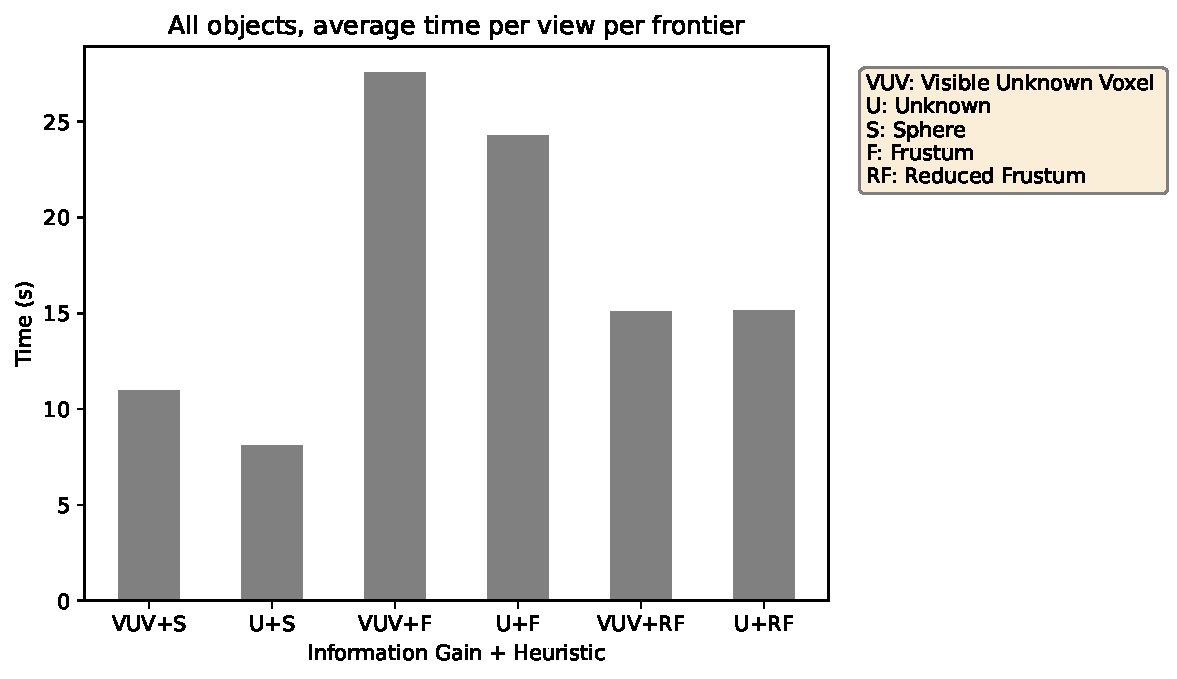
\includegraphics[width=0.6\textwidth]{Graphics/all_avg_times_frontiers.pdf}
\end{frame}

\begin{frame}{Experimente: Ergebnisse}
	\centering
	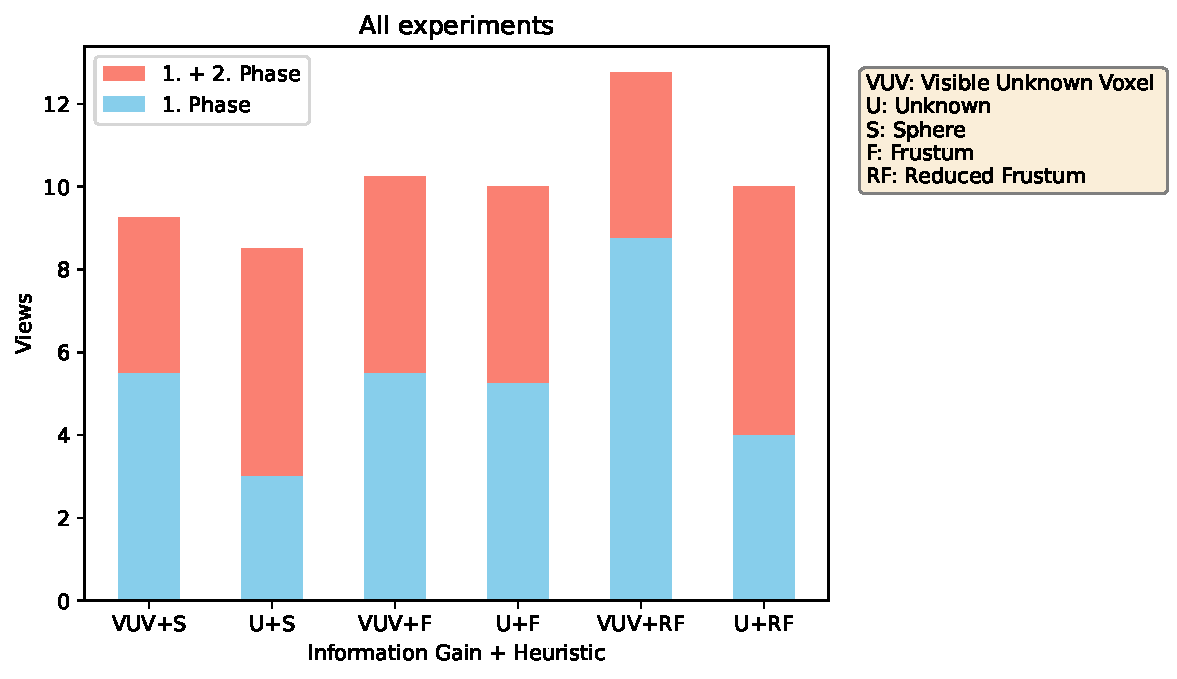
\includegraphics[width=0.9\textwidth]{Graphics/all_num_views.pdf}
\end{frame}


\begin{frame}{Experimente: Ergebnisse}
	\centering
	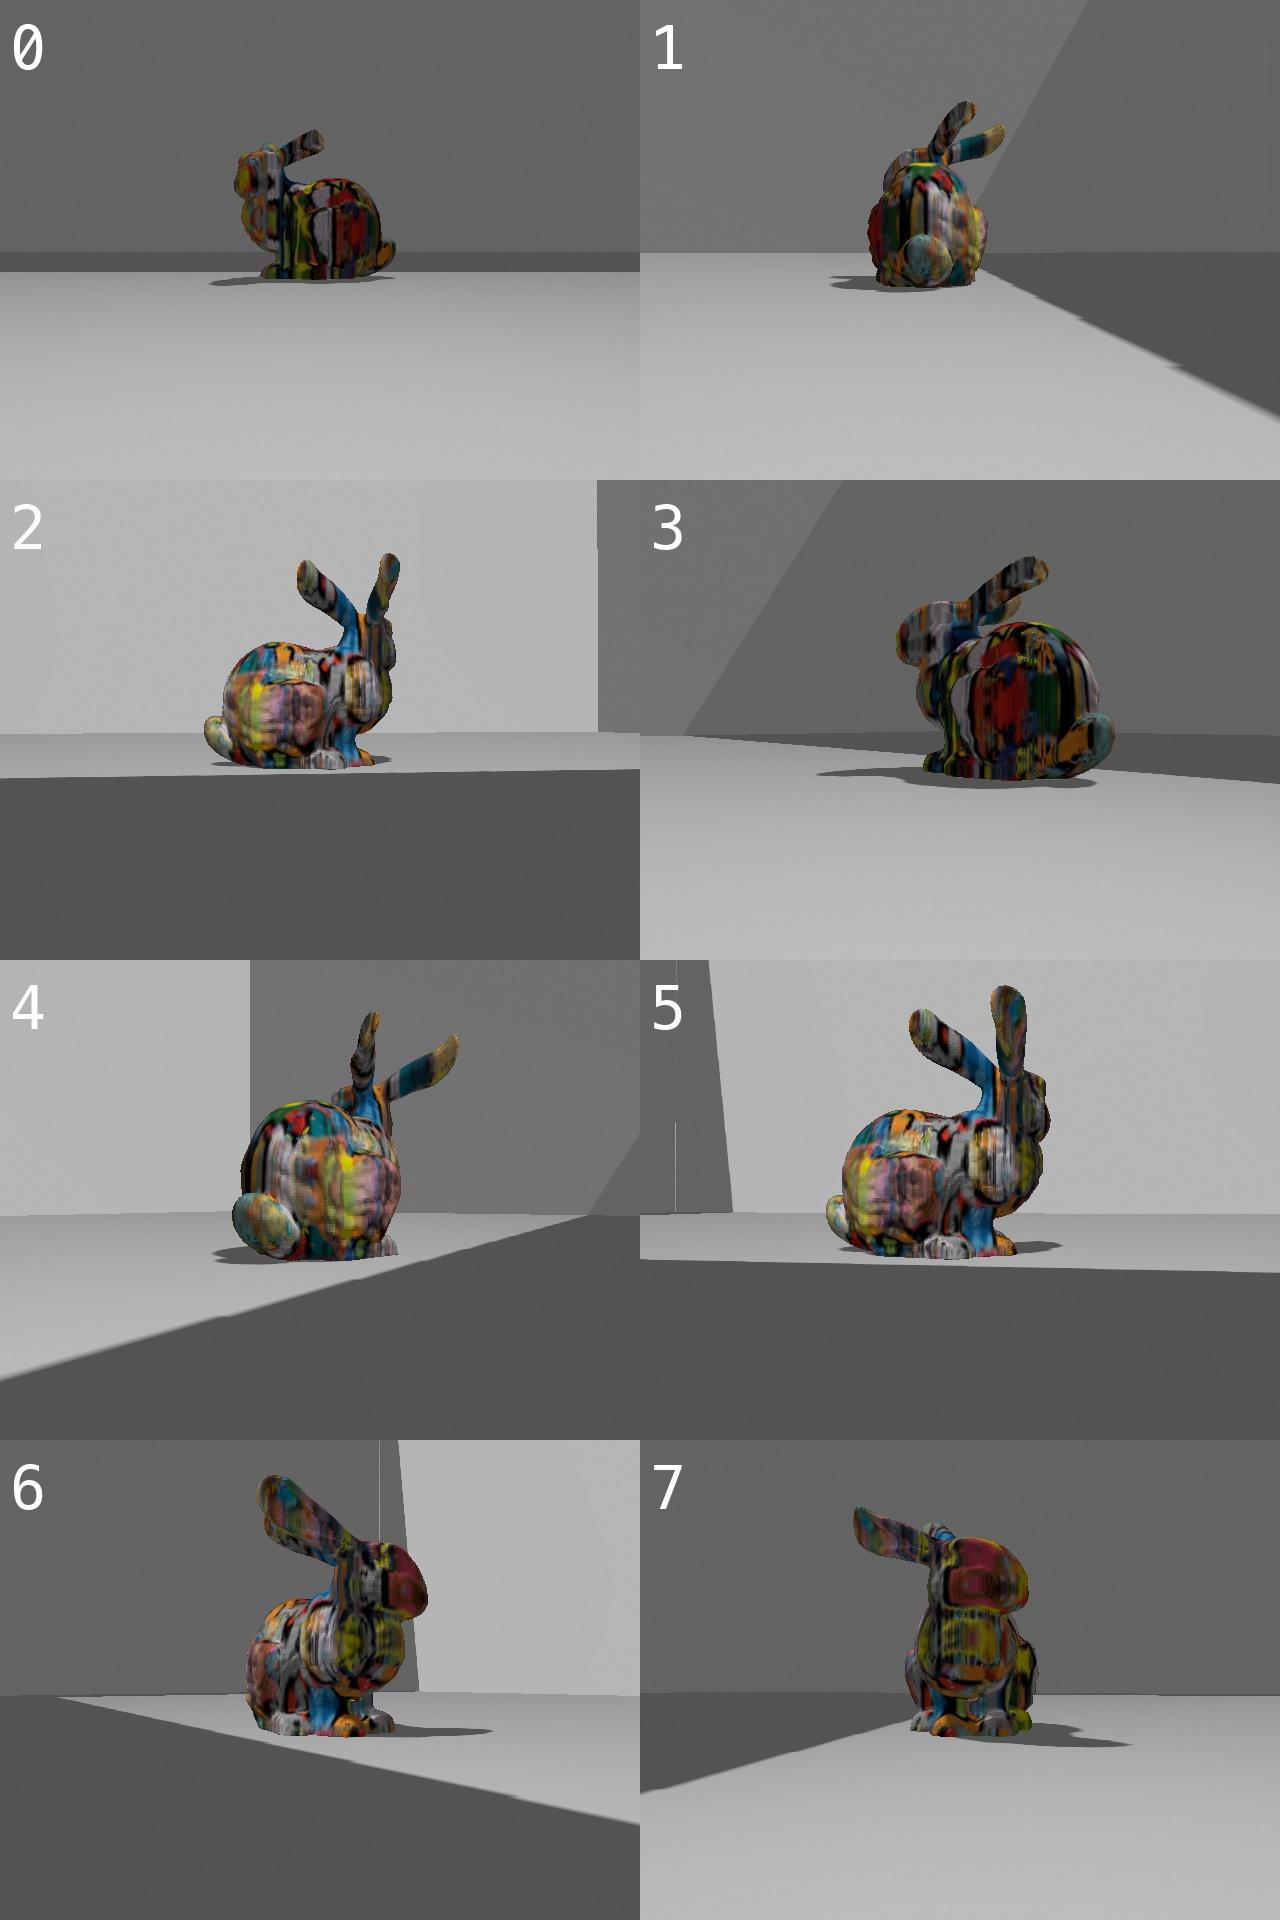
\includegraphics[width=0.4\textwidth]{Graphics/bunny_unknown_0_collage.jpg}
	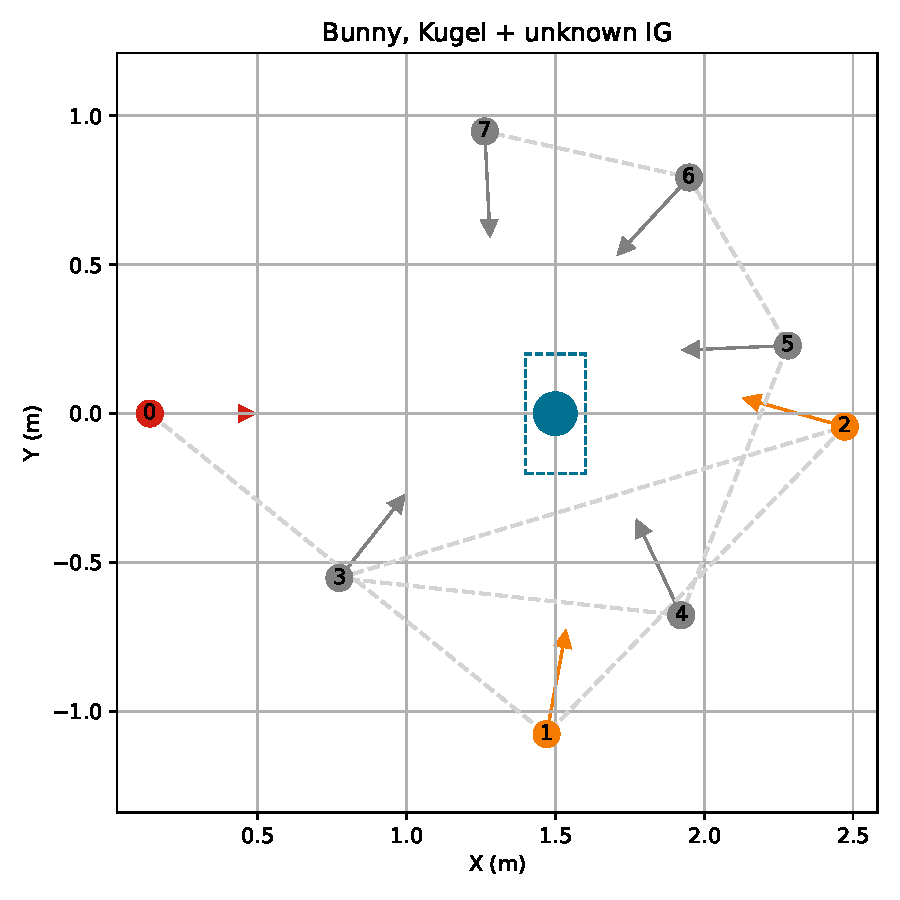
\includegraphics[width=0.59\textwidth]{Graphics/bunny_sphere_unknown_views.pdf}
\end{frame}

\begin{frame}{Herausforderungen und Ausblick}
	\begin{block}{Herausforderungen}
		\begin{itemize}
			\item VDB map: Unbekannte voxel in bereits bekanntem Gebiet
			\item Heuristiken unvorteilhaft gewählt
			\item Abbruchkriterien
		\end{itemize}

	\end{block}

	\begin{exampleblock}{Ausblick}
		\begin{itemize}
			\item Eigene Implementierung von VDB für den use-case angepasst
			\item Bessere Heuristik, z.B. Kugel mit Zentrum der bekannten Voxel oder Object Detection BBox
			\item Vergleich mit state-of-the-art Algorithmen
			\item Port auf realen Roboter wie Spot
		\end{itemize}
	\end{exampleblock}

\end{frame}

\begin{frame}{}
	\centering
	\Large{Danke für die Aufmerksamkeit!}
	\vfill
	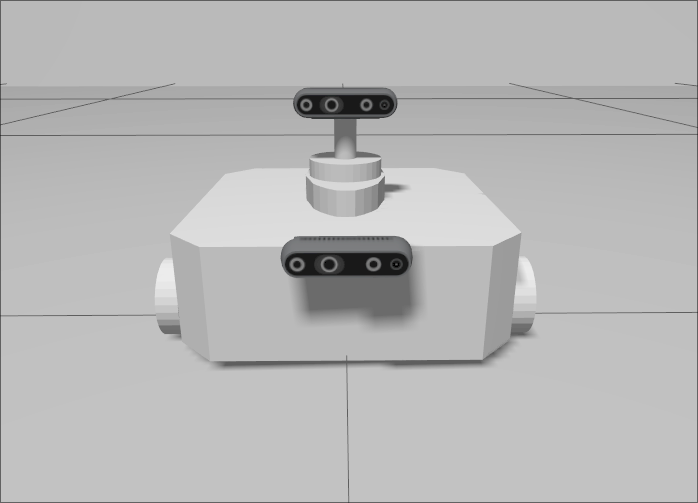
\includegraphics[width=0.5\textwidth]{Graphics/tb.png}
\end{frame}

\printbibliography
\end{document}
